
{\color{blue}4-28-16: The mean-field approximation and its limitations}

Recall the self-consistency or variational equation $M=\tanh(\beta J M + \beta h)$. 

For $\beta, J=1$, $t=\frac{\beta - \beta_c}{\beta_c}$, $\beta J = 1+\frac{\beta - \beta_c}{\beta_c} \beta_cJ = 1+t$, $M=\tanh(M+tM+h)$.

Recall that $\tanh(x) = x-\frac{1}{3}x^3 + O(x^5)$. In the vicinity of $(\beta_c,0)$, at $\beta = \beta_c$ ($t=0$), $M\approx M+h- \frac{1}{6} M^3 + \cdots$, $M(\beta, h) \approx (6h)^{\frac{1}{3}}$, $\boxed{\delta = 3}$. 

At $h=0$, $M\approx M-\frac{1}{6} M^3 + tM + \cdots$ %tlo.
We get $M^2 \approx 6t$, $M\approx (6t)^{\frac{1}{2}}$, and $\boxed{\widehat{\beta} = \frac{1}{2}}$.

For the magnetic Ising model in any dimension, we have inequalities. The bounds saturate in high dimensions.

For the finite range interactions, the critical exponents are correct for $d>4$, are correct with log corrections for $d=4$, and are wrong for $d<4$.

%shed light but misleading.
Another situation where mean-field theory applies (but is somewhat misleading) is hysteresis. Apply a magnetic field, and observe the time dependent magnetic field. At low enough temperature, when $h$ goes from $h>0$ to $h<0$, it doesn't drop immediately, and when $h$ goes from $h<0$ to $h>0$, it doesn't increase immediately.

\begin{center}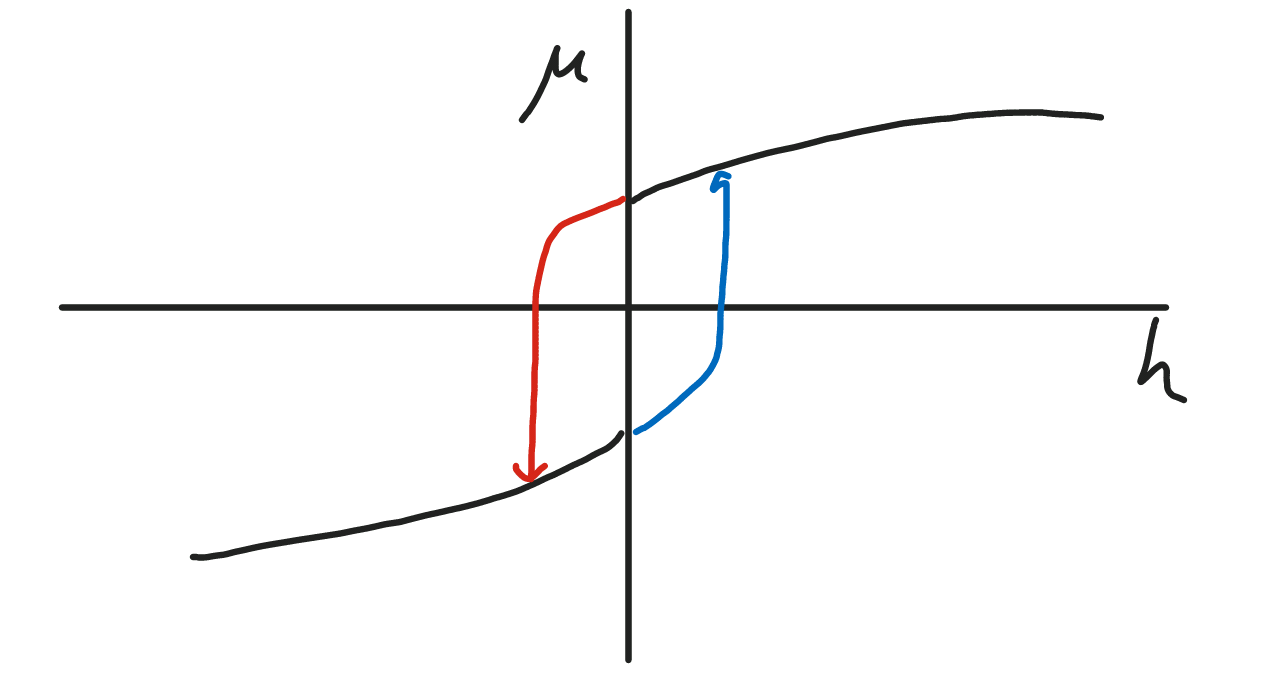
\includegraphics[scale=.25]{images/hys}\end{center}

This is a phenomenon of meta-stability.
%hold crystal, shake release.
One tempting idea is to explain this with the mean-field model.

Let 
\be\mu(\beta,h)=\operatorname{argmax}\Big\{\rho(M)+\underbrace{\frac{\beta}{2}M^2}_{\mathcal{E}(M)} + \beta hM\Big\}.\ee
%when $h$ starts to turn negative. Initially the function looks concave. Initially you think that it brings down the slope.
This occurs when 
\be
\frac{\partial}{\partial \mu} [\rho(M) + \mathcal{E}_0(M)] = -\beta h.
\ee
%brings down the slope of one part of the function.

But we cannot account for metastability using this.

\begin{theorem}[S.N. Isakov (Mathematical Physics, 1984)]
For the short-range Ising model on $\mathbb{Z}^d$, for any $d>1$, $M(\beta, h)$ has no analytic continuation in $h$ past $h=0$.
\end{theorem}
Often when a function is discontinuous, we can still extend it, perhaps on a different Riemann sheet; this is not the case here.

The growth rate of free energy implies zero radius of convergence.

This is conjectured to be a general feature (M.E. Fisher, Andreev 1964). 

Kac proposed to study the potential of long-range systems. The Kac potential is 
\begin{align}
J_x(\xi) &= \frac{1}{\xi^d}\varphi\left( {\frac{x}{\xi}} \right)
\end{align}
For some constant $C$,
\begin{align}
\int_{\mathbb{R}^l} J_x\,d^Dx &=C.
\end{align}

The free energy converges to mean field free energy.

\begin{theorem}
For the Kac potential on $\mathbb{Z}^D$, 
\be
\lim_{\xi\to \infty} \Psi(\beta, h;\xi) = \Psi_{MF} (\beta, h).
\ee
\end{theorem}

Neverthless, it is expected that the critical exponents do vary with $\xi$.
%correlations have divergent length scales.
%cross-over phenomenon.

%two more topics.



\section{Scaling limits}
The following 3 topics (scaling limits, stochastic geometry at the cricial point, and random fields) all have to do with behavior at the critical point. There is a line of first-order phase transition at the end of which there is a second-order phase transition.

The behavior of the system at large-scale is independent of local interactions.

At $h=0$, $\left\langle {\sigma_x}\right\rangle_{h,T}=0$, on a microscopic scale.
\begin{align}\label{eq:sl-corr}
\left\langle {\sigma_x\sigma_y}\right\rangle &\approx \begin{cases}
A e^{-|x-y|/\xi},&T>T_c\\
\frac{C}{|x-y|^{D-2+\eta}},&T=T_c
\end{cases}
\end{align}
where $\xi$ is the lattice correlation or ``mass."
At 2 points at a larger, intermediate (mesoscopic) scale, interaction is very weak. The natural thing is not to consider interactions between individual spins, but take a local average over spins. 

Let $x,y$ be points whose spacing is on the bulk scale. 
We are essentially looking at 
\be
S(x,y):=\left\langle {\sigma_{\left\lfloor\frac{x}{a}\right\rfloor}, \sigma_{\left\lfloor\frac{y}{a}\right\rfloor}}\right\rangle\underbrace{\frac{1}{\left\langle {\sigma_0\sigma_{\left\lfloor\frac{L}{a}\right\rfloor}}\right\rangle}}_{C(L)}.
\ee
We are thinking of $x$ as a lattice point on a lattice with very fine mesh, $x\approx a\left\lfloor\frac{x}{a}\right\rfloor$ with $\left\lfloor\frac{x}{a}\right\rfloor\in \mathbb{Z}^D$. 

Let $L$ be the distance of the scale at which we want to probe the system. 

%corre function on macroscopic scale.
%choose some macroscopic scale. 
%what would happen to the rest of the function?
%take exp function, normalize it, 

We have an exponential function which decays with respect to the lattice spacing with some fixed factor. When you look at it, normalized on the lattice scale so that $S=1$ at $L$, then $S=\infty$ when at $<L$ and $S=0$ at $>L$.

We have
\be
\lim_{a\searrow 0} S_{a;L} (x,y) =
\begin{cases}
\infty,&|x-y|<L\\
0,&|x-y|=L\\
1, &|x-y|>L.
\end{cases}•
\ee
This is boring.
But something different happens when you have a power law. When you half the distance, you multiply the function by a constant.

At $T=T_c$, $h=0$, assuming~\eqref{eq:sl-corr},
\be
S_{a,L}(x,y) \to \left( {\frac{L}{|x-y|}} \right)^{D-2+\eta}
\ee
Considering local averages, we can talk about joint distribution of averages of spins.

In an optimistic yet credible scenario, $\lim_{a\searrow 0}$ exists for rescaled spin variables
\be
\psi(x) = \frac{1}{a^*} \sigma_{a\left\lfloor\frac{x}{a}\right\rfloor}
\ee
%what ask for, what makes no sense.
%joint dist
in the distributional sense.

Take a smooth function $g(x)$ of compact support. Define the function 
\be\Psi(g)\stackrel{D}= \lim_{a\searrow 0} \int g(x)\frac{1}{a^{\#}} \sigma_{a\left\lfloor\frac{x}{a}\right\rfloor} \,d^Dx.
\ee
%Riemann approximation. sum over lattice vars with right weight.
%it's a lot of work to prove that ... exists
%
(This is interpreted as a Riemann sum over the lattice.)
The notation means we are taking a distributional limit.
Such limits make sense. We construct what we refer to as a field. It's not a function. It's a random entity. It should not be thought of as defined at every single point, but should be thought of as defined throughits integral with smooth functions.

At the microscopic level, spins fluctuate---there is an uncountable amount of information! But if we care about functions which on the scale of the continuum are smooth, we don't need this information. 
%It's not that the values...

When we say the random field is a distribution, we say that the integral for a certain space of smooth functions this makes sense. (Actually smoothness is not essential.)

We have
\begin{align}
\mathbb{E}\left( {\left| {\int_{|x|\le L} \psi(x)\,dx} \right|^2} \right)
& = \int_{|x|,|y|\le L}
\mathbb{E}(\psi(x)\psi(y))\,dx\,dy \\
&= \lim_{a \searrow 0}\frac{a^{2D}}{a^{2\#}} \sum_{|u|,|v|\le \frac{L}{a} }\left\langle {\sigma_u\sigma_v}\right\rangle\\
&\approx \lim_{a\searrow 0} a^{2(D-\#)}\left( {\frac{L}{a}} \right)^{2D} \left( {\frac{a}{L}} \right)^{D-2+\eta}\\
& = \frac{L^{2D}}{L^{D-2+\eta}}.
%variable construct has a finite second moment.
%
\end{align}
%$\lim_{a\searrow a^{....}}$.
Consider the average block spin, scaled up so that we are looking at it on its scale of typical fluctuation. What is the distribution of these block variables? Field theory describes the distributions.

For a long time, there was the field theory project.

We expect interactions in physics to be local. How do local interactions build meaningful interactions over large distances? They produce interesting interactions only at criticality; otherwise there is exponential decay. 

There was a meeting of minds between statistical physicists and high-energy physicists.

Here we have a negative result.
\be
S_n(x_1,\ldots, x_n)=\lim_{a\searrow 0} \frac{1}{a^{n\#}} \left\langle {\prod_{j=1}^n \left( {\sigma_{a\left\lfloor\frac{x}{n}\right\rfloor}} \right)}\right\rangle.
\ee
define
\be
U_n 
\ee

\begin{theorem}
Ising models in $D>4$ dimensions in the scaling limit ($T=T_1,h=0, a\searrow 0$), adjusted so $S_2(x,y)$ converges, satisfies 
%converge
%converge to Gaussian.
\be
\lim_{a\to 0}
\frac{S_n(x_1,\ldots, x_n)-\sum_{\text{pairings }\pi} \prod_{j=1}^{\frac{n}{2}} S_{2,a}(x_{\pi(2j-1)}, x_{\pi(2j)})}{S_{n,a}(x_1,\ldots, x_n)}=0.
%monotone permutations
\ee
\end{theorem}
%sum over lattice animals.
%statistical distribution percolate.

%The two-point . Line with endpoints $x,y$.
%effect on free energy

The $n$-point functions can be understood as walks (actually clusters with dangling things which may scale into walks). There's a way of geometrizing the problem. 

Beautiful math developments.

%We consider random 2-dimensional surfaces

%\section{Stochastic geometry at the critical point}
%
%\section{Random points}

